\section{YAFFS2 Results}

\begin{figure*}[t]
  \centering
  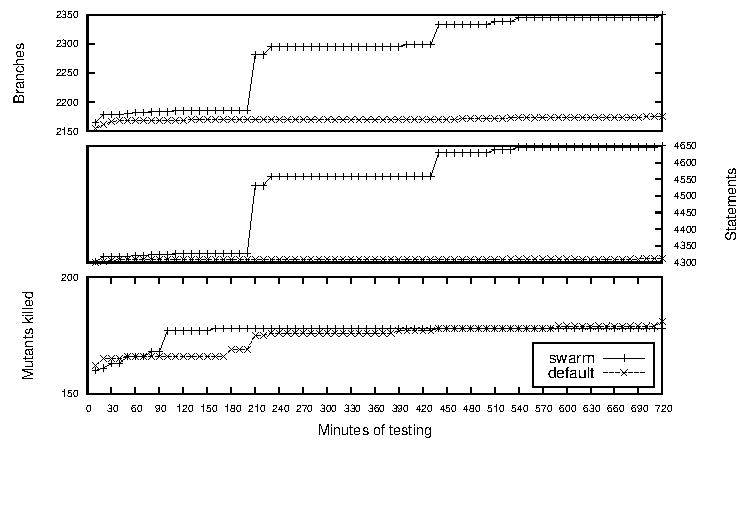
\includegraphics[width=\textwidth]{../graphs/yaffs2/yaffs2}
  \vspace{-1.3in}
  \caption{YAFFS2 Results}
  \label{fig:yaffs2}
\end{figure*}

YAFFS2~\cite{yaffs2} is a popular open-source NAND flash file system
for embedded use; it was the default image format for early versions
of the Android operating system.  The test generator for YAFFS uses 47
different API calls as features.  Applying swarm testing to YAFFS2 was
essentially trivial, as the capability to turn on or off API calls is
natural to such API-based random test generators; we did refactor the
control from a {\tt \#define} based approach to command-line
parameters to ease use of swarm testing.

Figure \ref{fig:yaffs2} shows that swarm testing improves not only
branch and statement coverage but also mutation kill rates for YAFFS2.
Because YAFFS2 is a smaller and simpler program than SpiderMonkey, we
used 10 minute rather than 30 minute test intervals.  All differences
between swarm and default testing were statistically significant by
Wilcox U-test for the 10 minute intervals, with $p$-values of $3.1
\times 10^7$ or lower.  Tables \ref{tab:yaffseffect} summarizes 95\%
confidence interval absolute gains in coverage and mutation kill for 10 minutes of swarm testing vs. 10 minutes of default testing.

\begin{table}
\caption{95\% effect sizes (absolute) for swarm over default, YAFFS2}
\centering
\begin{tabular}{c|c|c}
\hline
ST & BR & Mutants Killed \\
\hline
\hline
15.7 - 50.1 & 10.5 - 28.1 \\
\hline
\end{tabular}

\label{tab:yaffseffect}
\end{table}
